\subsection{Ruangan Kafe (\emph{Cafe World})}
\label{subsec:lingkunganindoor}

Ruangan kafe (\emph{cafe world}) dibuat dengan menyusun \emph{file} SDFormat yang berisi ruangan tertutup dengan berbagai macam objek di dalamnya.
Seperti yang terlihat pada potongan kode \ref{lst:indoorworldsdf},
  ruangan virtual ini terdiri atas objek pencahayaan dan \emph{include file} pada \emph{path} \lstinline{model://cafe}, \lstinline{model://cafe_table}, \lstinline{model://dienen_robot}, dan \lstinline{model://dienen_human}.
Dua \emph{path} pertama merupakan \emph{path} dari model yang sudah disediakan oleh Gazebo,
  yang membentuk ruangan kafe beserta perabotan yang ada di dalamnya,
  sedangkan dua \emph{path} terakhir merupakan \emph{path} dari model robot dan model pengguna yang sebelumnya sudah dibuat di bagian \ref{sec:modelrobot} dan \ref{sec:modelpengguna}.

\lstinputlisting[
  language=XML,
  style=code,
  caption={Struktur SDFormat dari ruangan kafe (\emph{cafe world}).},
  label={lst:indoorworldsdf}
]{kode/sdf/indoor_world.xml}

Setelah \emph{file} SDFormat dibuat,
  hasil yang didapatkan setelah dijalankan pada simulator tampak seperti pada gambar \ref{fig:lingkunganindoor}.
Sesuai dengan susunan yang diisi pada \emph{file} SDFormat,
  tampak adanya model robot dan pengguna di dalam sebuah ruangan kafe dengan berbagai macam perabotan yang ada di dalamnya seperti meja, lemari, jendela, dan lain sebagainya.

\begin{figure}[ht]
  \centering
  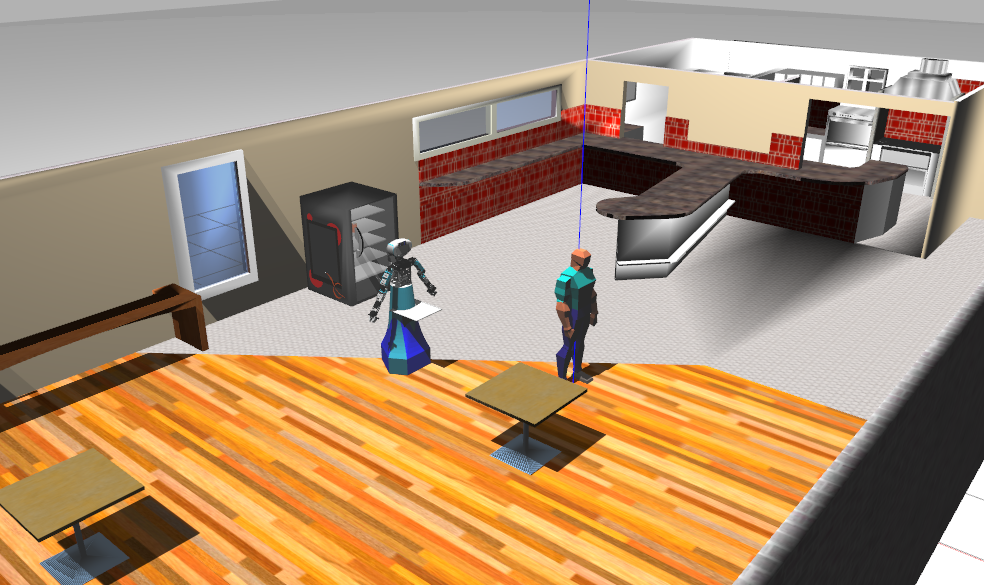
\includegraphics[scale=0.23]{gambar/lingkungan-indoor.png}
  \caption{Tampilan ruangan kafe (\emph{cafe world}) pada Gazebo.}
  \label{fig:lingkunganindoor}
\end{figure}
